\section{Spettro di emissione delle galassie}\label{sec:spettro-di-emissione-delle-galassie}
\subsection{Caratteristiche generali}
Per osservare le galassie viene ovviamente raccolta la radiazione proveniente da loro, ma essendo corpi celesti molto lontani otteniamo delle immagini spesso poco soddisfacenti, perché non è possibile distinguere le singole stelle che compongono la galassia (in quel caso si dice che stiamo osservando una popolazione stellare risolta). Per le galassie più lontane, per le quali la magnitudine non è risolvibile, la magnitudine è la cosiddetta \emph{magnitudine integrata} di tutte le stelle al suo interno: quello che osserviamo quindi è la cosiddetta luce integrata, che viene dalla somma di sorgenti non risolte per la maggior parte delle galassie (solo le stelle delle galassie del Gruppo Locale sono risolte, per le altre no). Allo stesso modo della luce, possiamo osservare che anche il colore di una galassia lontana è dato dall'integrale dei colori delle singole stelle e allo stesso modo possiamo applicare il medesimo ragionamento anche per uno spettro di risoluzione $\Delta\lambda$ finita. Quindi quando osserviamo la luce proveniente da una galassia in realtà stiamo osservando la luce che viene da diverse fonti: fluso o magnitudine integrata, colore integrato e spettro integrato con risoluzione $\Delta\lambda$ finita. Le normali tecniche di risoluzione stellare NON sono applicabili a galassie lontane.

Data una galassia, la luce che osserviamo provenire da essa sarà sicuramente emessa dalle stelle che la compongono ma non solo, abbiamo diverse origini:
\begin{itemize}
    \item Stelle: emissione fotosferica (UV - infrarosso intermedio), vento stellare (linee di emissione, IR da involucri di polvere), fenomeni di accelerazione (raggo X binari).
    \item Gas: freddo (idrogeno non ionizzato, nubi molecolari), tiepido (T $\sim$ $10^4$ K, linee di emissione, idrogeno ionizzato), più tiepido (T $\sim$ $2-3 10^4$ K, resti di supernovae, compressioni rapide del gas), caldo ( T $\sim$ $10^7$ K, raggi X, linee di emissione continua).
    \item Polvere: emissione termica (luce stellare riprocessata dalle interazioni, shock termico), caratteristiche di emissione/assorbimento (PAHs, silicati e grafiti), scattering (UV - luce infrarossa).
    \item Nucleo Galattico Attivo (AGN): non è presemte in tutte le galassie, si tratta di un buco nero supermassiccio al centro di una galassia. Ci può essere emissione termica e non termica (spettro continuo e discreto). Nell'emissione termica lo spettro principale è quello dalle onde radio ai raggi gamma. La radiazione di un AGN può dominare l'intero spettro integrato.
\end{itemize}

In figura~\ref{fig:spettro+galassie} è riportato lo spettro di emissione (per lunghezza d'onda) delle galassie divise per morfologia: possiamo notare che determinate emissioni con una lunghezza d'onda precisa sono proprie della formazione stellare (osserviamo dei picchi in corrispondenza di quelle $\lambda$, come per OII e H$\alpha$) e infatti non appaiono in spettri di galassie in cui non si ha generazione stellare (passive, come quelle ellittiche o lenticolari). Lo spettro prende tutte le galassie; si potrebbe anche osservare la distribuzione spettrale di energia (SED) di una galassia in cui si verifica formazione stellare, che riporta solo un campionamento. Il confronto tra i due grafici (l'altro è sulle slide) è però in accordo con quanto riportato, si osservano quei picchi in entrambi i casi.

\begin{figure}
    \centering
    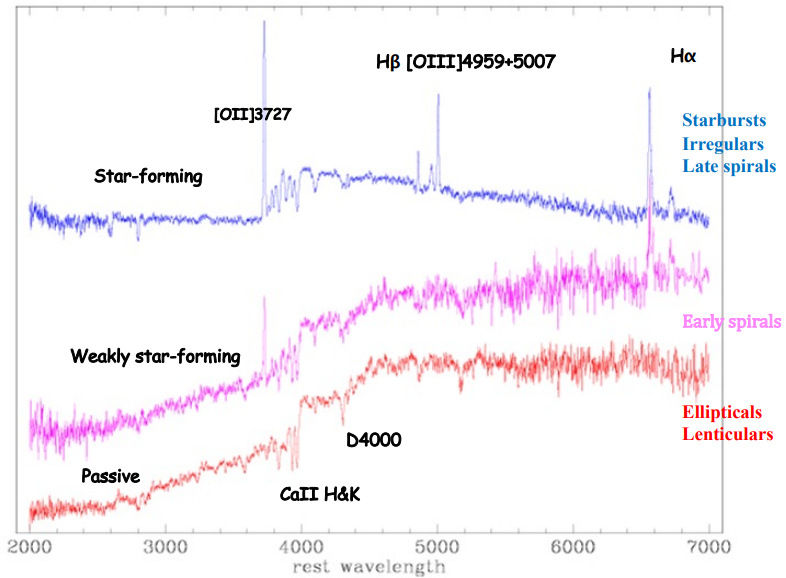
\includegraphics[width = 0.5 \textwidth]{immagini/spettro-galassie.png}
    \caption{Lo spettro della radiazione diviso per morfologia mostra come alcune lunghezze d'onda siano specifiche per galassie in cui si verifica formazione stellare}
    \label{fig:spettro+galassie}
\end{figure}

\subsection{Gas freddo, gas tiepido e polvere nelle galassie a spirale}
Come abbiamo detto una parte della radiazione proveniente dalle galassie proviene da gas freddo, in particolare da idrogeno neutro (H I); questo all'interno di una galassia è caratterizzato da una densità superficiale $ \sim 1 -\SI{10}{\solarmass.pc^{-2}}$, con un disco di dimensioni circa 5 volte maggiori dei dischi stellari (arriva fino a $\sim 100 Kpc$). L'idrogeno neutro si osserva in banda radio, dal momento che l'emissione è di radiazione a lunghezza d’onda pari a $21$ cm. Perché avviene l'emissione? Si tratta di una transizione dovuta alla struttura iperfine dell’atomo di idrogeno. Il livello fondamentale dell’atomo di idrogeno è diviso in due sottolivelli: nel livello di più bassa energia il protone e l’elettrone hanno spin opposto, mentre il livello in cui gli spin sono uguali ha energia lievemente superiore (differenza di $6*10^{-6}eV$, corrispondente alla lunghezza d’onda di $21$ cm). Questa transizione è impossibile sulla Terra, avendo probabilità di emissione molto bassa, che corrisponde ad un'emivita lunghissima ($\tau \sim 10^7$ anni). Tuttavia, osserviamo tale transizione nell’universo a causa dell’elevata abbondanza di idrogeno, infatti la linea di emissione a $21$ cm è ben visibile sia per la Via Lattea, sia per altre galassie più esterne. La distribuzione di idrogeno neutro, inoltre, non è uniforme nel disco galattico: si ha infatti una zona di maggior densità (uguale per idrogeno ionizzato) lungo i bracci della spirale della galassia. 

L'idrogeno può comparire anche a temperature più alte e in quel caso si tratta di idrogeno ionizzato (H II): ci sono alcune regioni che si osservano in luce ultravioletta perché la radiazione viene emessa da stelle OB (stelle più calde – più giovani, hanno un'emissione così energetica che ionizza gas circostante, emettendo in banda UV). Stelle così calde si trovano in una zona di formazione stellare; osservare gas ionizzato è quindi indice della presenza di formazione stellare. Dal momento che questo fenomeno si osserva principalmente lungo i bracci della galassie, se ne deduce che i bracci delle galassie a spirale sono luogo di formazione stellare. 

Per quanto riguarda invece il gas freddo e la polvere, questi sono osservabili in luce infrarossa, perché  per assorbimento (reddening) della luce, questa viene riemessa in banda infrarossa. 
